\chapter{Functional Verification of Sequential Normal Basis Multiplier}
\label{ch:normal}
In order to utilize our traversal algorithm, it is necessary to find out
a sort of suitable circuit benchmarks which is easy to compute its
Gr\"obner basis (GB). From the work of {\it Lv} \cite{lv:phd},
we learn that arithmetic circuits in Galois field (GF) is
convertible to an ideal of circuit polynomials, and the 
ideal generators form a GB themselves when applying reverse topological
term order. Furthermore, according to the work of {\it Pruss et al.}
\cite{pruss:tcad15}, with a limited computation complexity,
we can abstract the word-level signature of an arithmetic 
component working in GF. Thus, we consider the possibility 
of applying our traversal algorithm on sequential Galois
field circuits. In each frame, we can use the techniques 
from \cite{pruss:tcad15} to abstract the word-level
signature of the combinational logic, which corresponds
to the transition function in our traversal algorithm.
As a result, we manage to find a type of sequential GF multiplier
which we can apply our traversal algorithm to actually 
verify its functional correctness.

\section{Motivation}
\label{sec:normal_motiv}
From the preliminaries about FSMs in Section \ref{sec:reach}, we learn that the
Moore machine does not rely on inputs for state transitions. 
As depicted in Figure \ref{fig:Moore}(a), a typical Moore machine implementation
consists of combinational logic component and register files, where
$r_0,\dots,r_k$ are present state (PS) variables 
standing for state inputs (SI), and $r_0',\dots,r_k'$ are next state (NS) variables standing for
state outputs (SO). Figure \ref{fig:Moore}(b) shows the state transition graph (STG) of 
a Moore machine with $k+1$ distinct states. We notice that it forms a simple chain,
with $k$ consecutive transitions the machine reaches final state $R_k$.

\begin{figure}[H]
\centering{
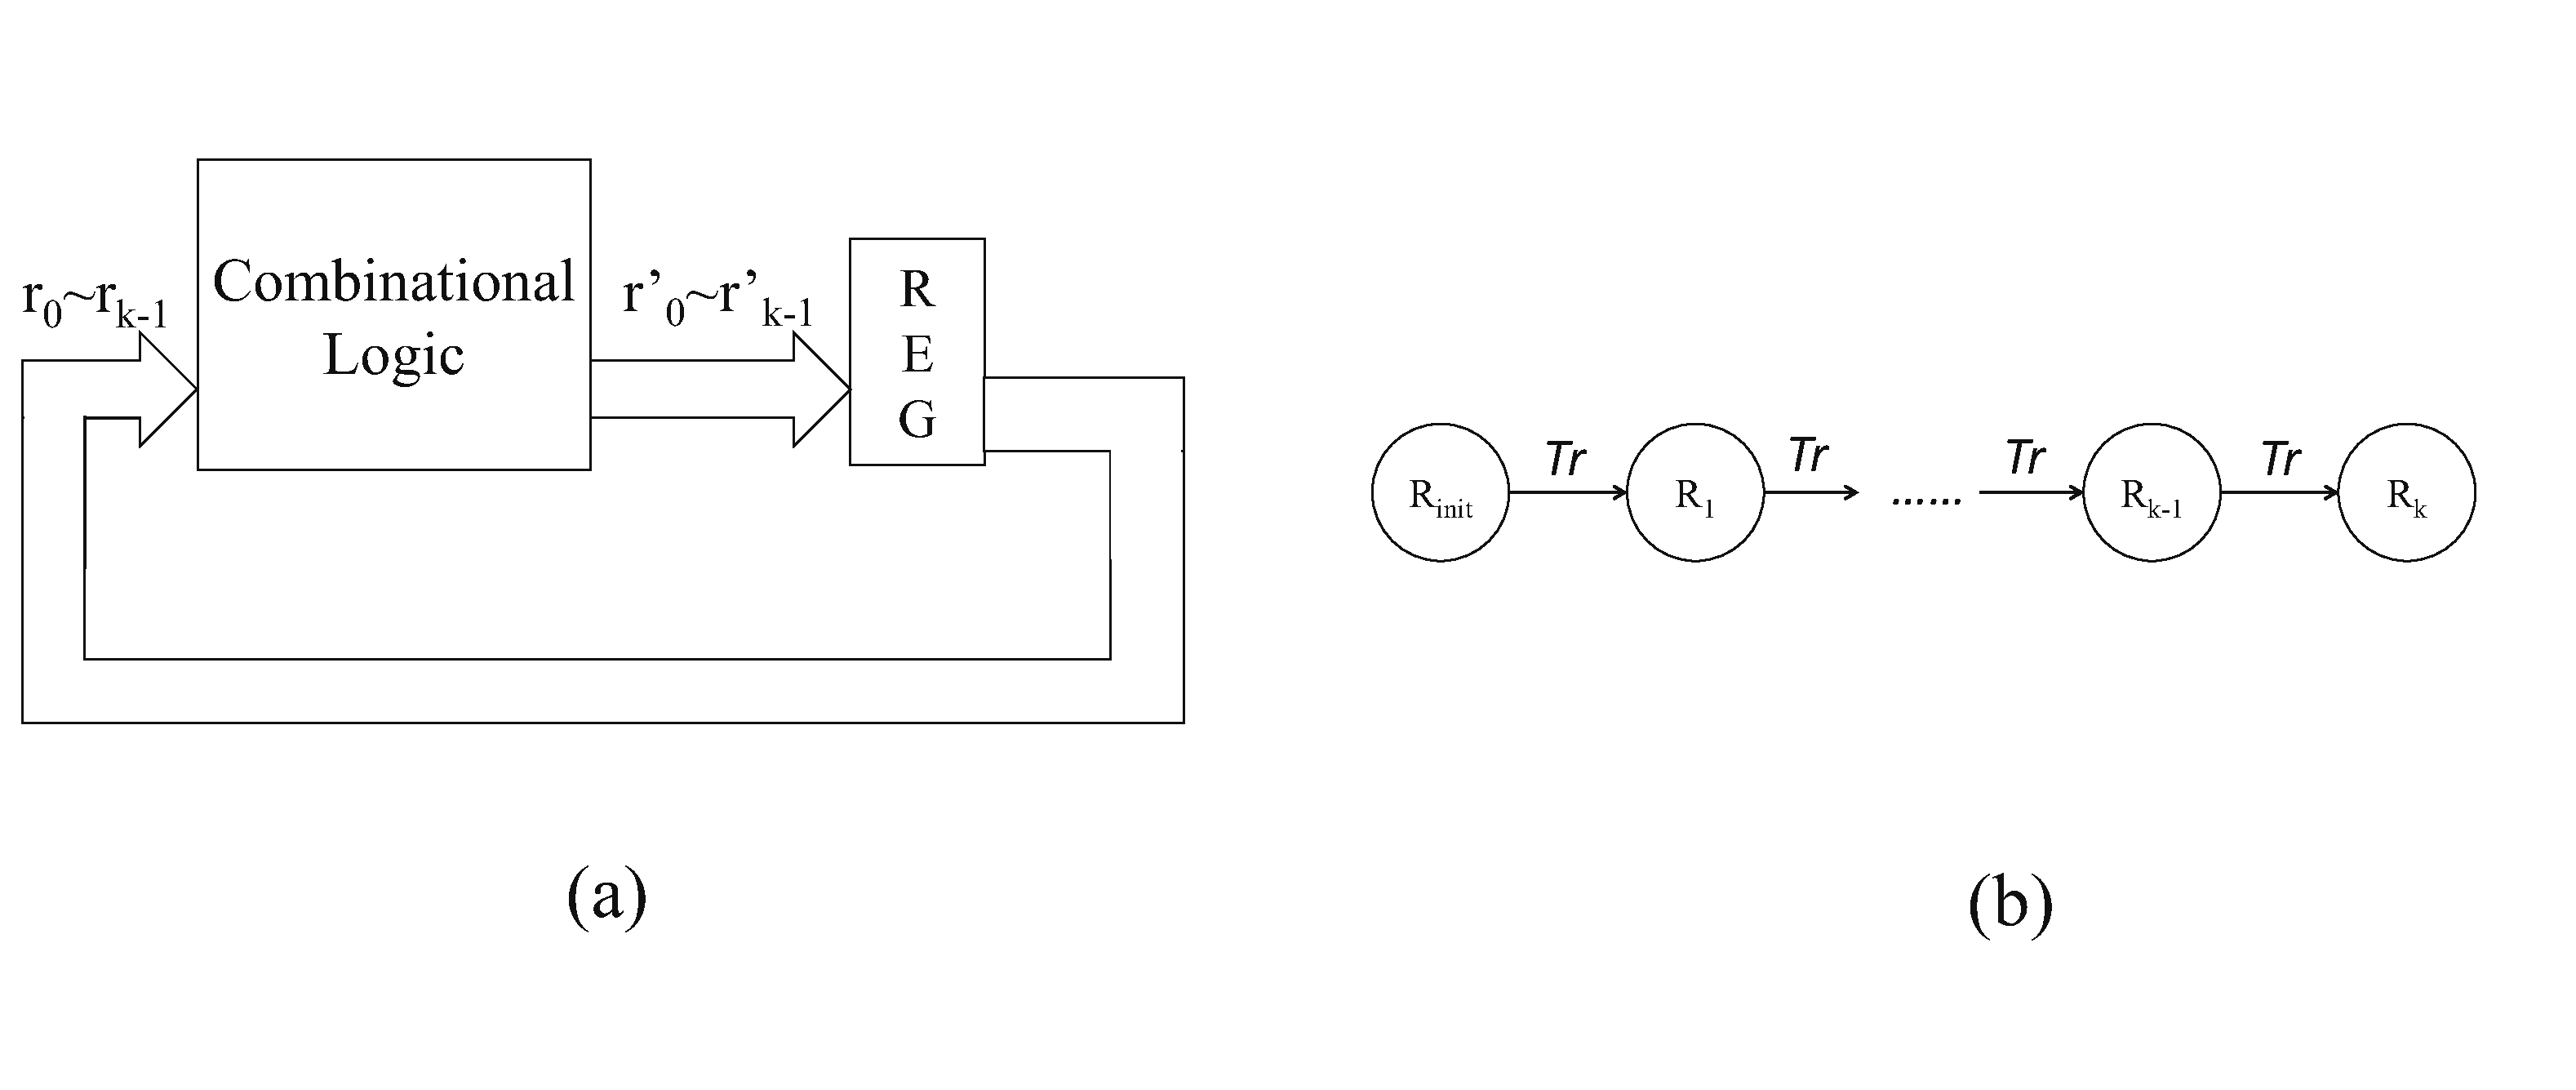
\includegraphics[width=\textwidth]{newfig/Moore.eps}
\caption{A typical Moore machine and its state transition graph}
\label{fig:Moore}}
\end{figure}

In practice,
some arithmetic components are designed in sequential circuits similar to the structure in 
Figure \ref{fig:Moore}(a). Initially the operands are loaded into the registers, 
then the closed circuit executes without taking any additional information from outside,
and store the results in registers after $k$ clock cycles. Its behavior can be described using
STG in Figure \ref{fig:Moore}(b): state $R$ denotes the bits stored in registers. Concretely, $R_{init}$ is the initial
state (usually reset to all zeros), $R_1$ to $R_{k-1}$ are intermediate results stored as SO of current state and SI
for next state, and $R_k$ (or $R_{final}$) is the final result given by arithmetic circuits (and equals to the answer
to arithmetic function when circuit is working functional correctly).
This kind of design results in 
reusing a smaller combinational logic component such that the area cost is greatly optimized.
An example of these designs is the sequential GF arithmetic multipliers described in Chapter \ref{ch:prelim_GF}.
However, it also brings difficulties in verifying the the circuit functions.

\begin{figure}[H]
\centering{
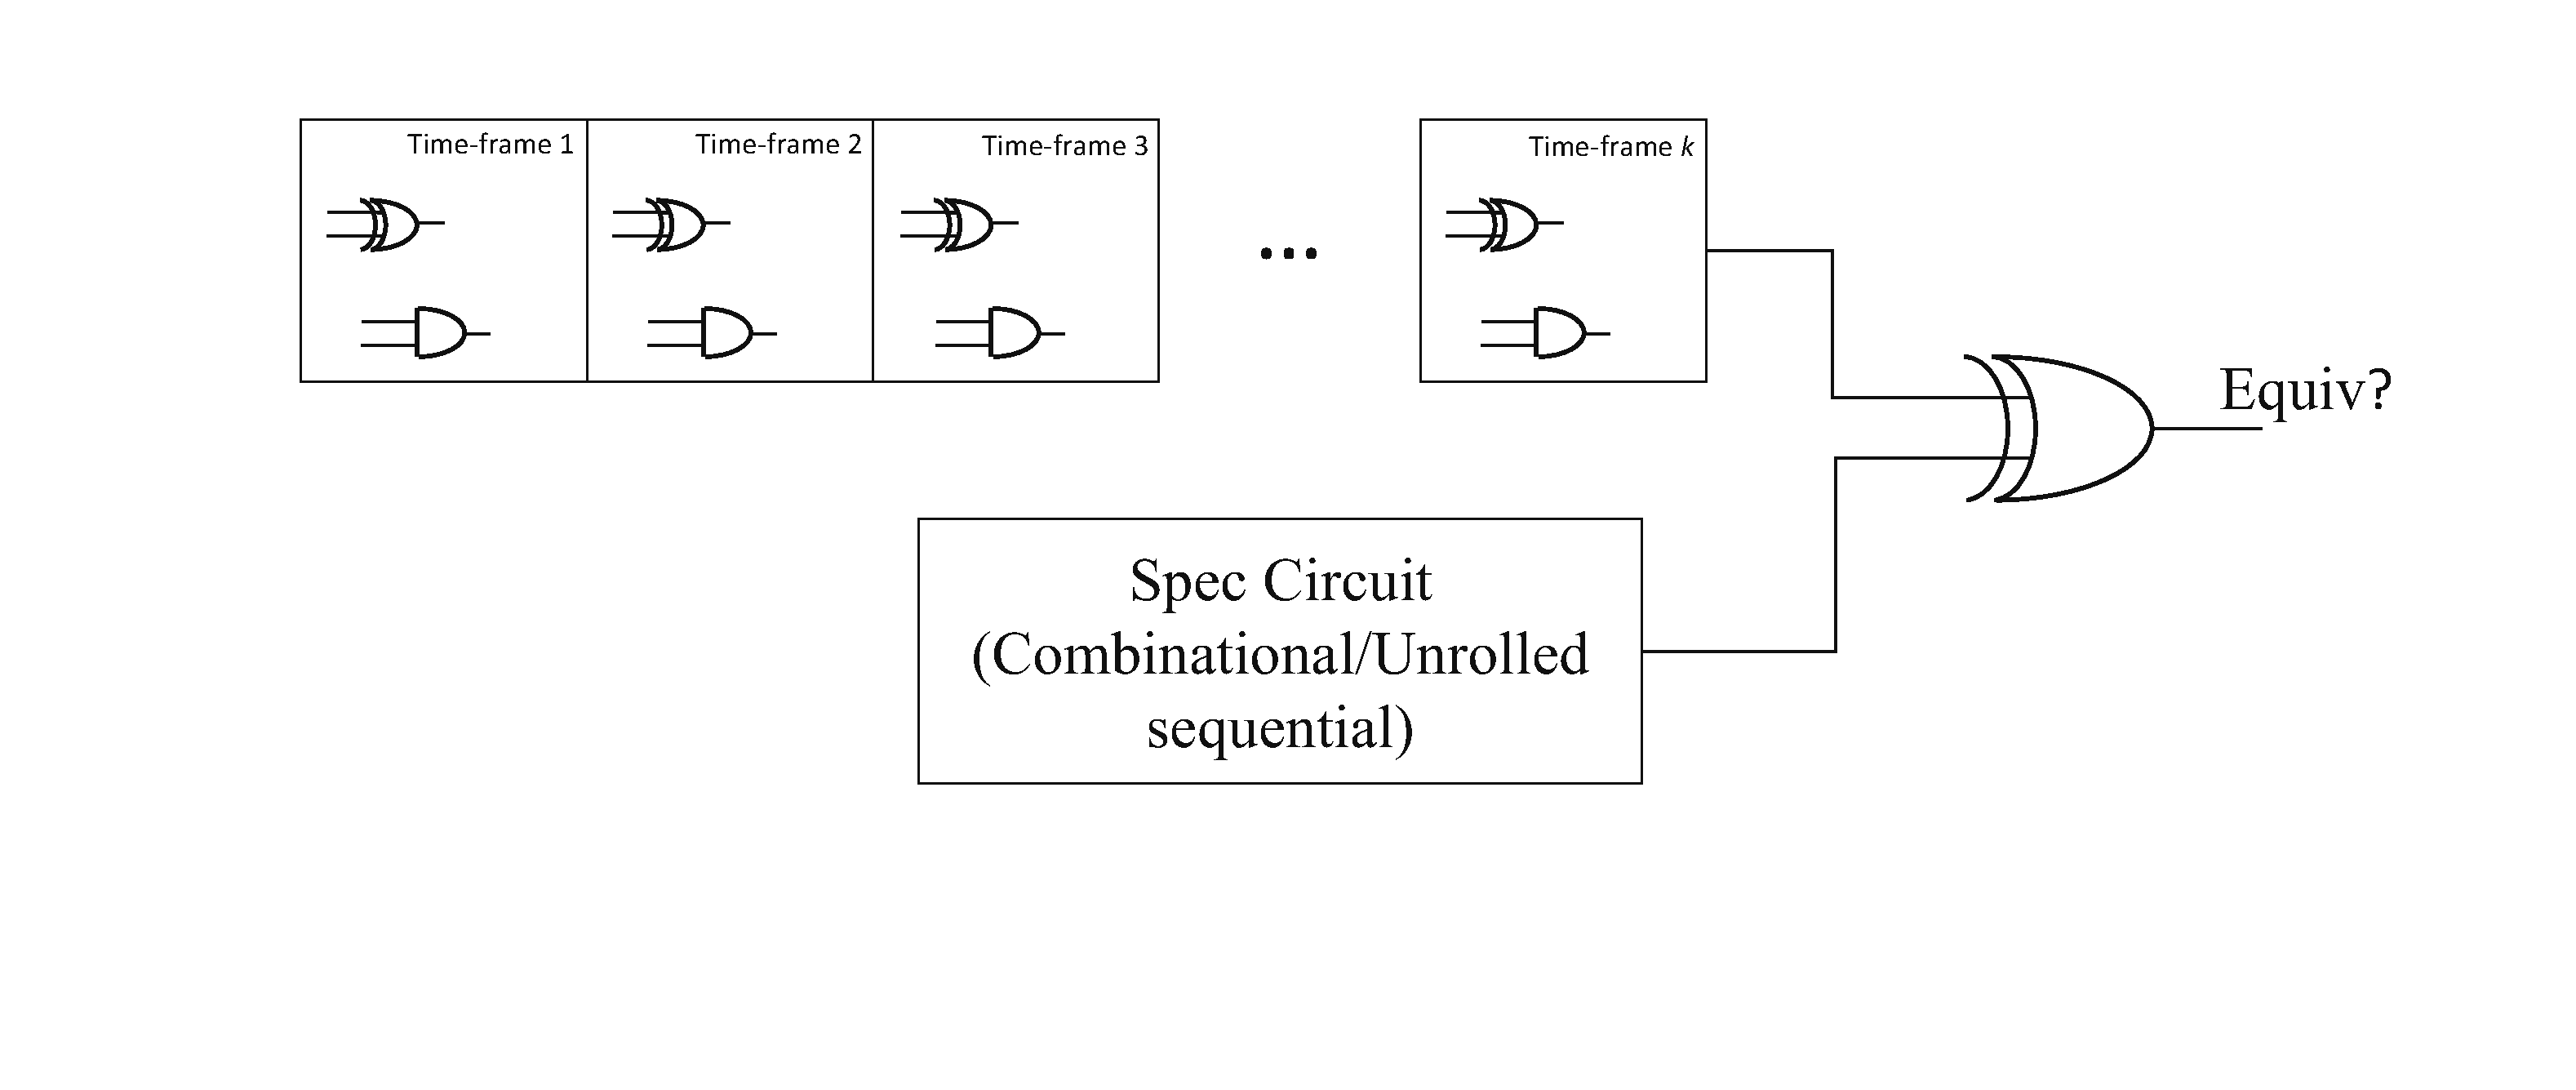
\includegraphics[width=\textwidth]{newfig/convention.eps}
\caption{Conventional verification techniques based on bit-level unrolling and equivalence checking}
\label{fig:convention}}
\end{figure}

Conventional methods to such a sequential circuit may consist of unrolling the circuit for 
$k$ time-frames, and performing an equivalence checking between the unrolled machine and
the specification function. However, the number of gates will grow fast when doing unrolling
on bit-level. Meanwhile the structural similarity based equivalence checking techniques 
will fail when the sequential circuit is highly customized and optimized from the naive specification 
function. As a result, conventional techniques is grossly inefficient for large circuits.
Therefore, a new method based on our proposed word-level FSM traversal technique is worthy to be explored.

\section{Formal Verification of Normal Basis Multiplier using Gr\"obner Basis}
The gate-level design of a NB multiplier can be generated using appoaches introduced in 
Section \ref{sec:nbdesign}. The gate-level netlist is ready to be verified using 
an approach similar to that in Chapter \ref{ch:reacha}. 
First we introduce the sketch of our approach using abstraction term order (ATO)
mentioned previously in Section \ref{sec:abstraction}, then refine our approach using 
the concept ``RATO", which is previously used in Section \ref{sec:improve}.
% The following part borrows contents
% from my own conference paper \cite{myDATE}.
\subsection{Implicit Unrolling based on Abstraction with ATO}
% fig:comb_RAB

The concept of abstraction was discussed in Section \ref{sec:abstraction}. If we use an elimination term order with
$intermediate~variables~>~R~>~A,B$ for the circuit in Figure \ref{fig:comb_RAB} to compute Gr\"obner basis, 
the function of the combinational logic component can be abstracted as 
$$R = \Func(A,B)$$
To verify the functional correctness of a combinational NB multiplier (e.g. Mastrovito multiplier
or Montgomery multiplier), the function given by abstraction will be computed as
$$R=A\cdot B$$
While in the sequential case, the function of combinational logic only fulfills a part of the multiplication.
For example, in the RH-SMPO introduced in Section \ref{sec:nbdesign}, 
the combinational logic actually implements  $F_{k-1}$ in Equation \ref{eqn:aux},
while computing all of $F_i$ requires $k$-cycle unrolling of the circuit.
Nevertheless, the abstraction still provides a word-level 
representation which can be more efficient for unrolling than bit-level expressions.
In other words, with the assistance of abstraction, we can execute implicit unrolling instead of 
explicit unrolling and avoid bit-blasting problem.

For 2-input sequential NB multipliers, abstraction is utilized to implement following algorithm:
%\vspace{-0.1in}
\IncMargin{1em}
\begin{algorithm}[hbt]
\SetAlgoNoLine
\LinesNumbered
 \KwIn{Circuit polynomial ideal $J$, vanishing ideal $J_0$, initial
   state ideal for output $R (=0)$, inputs $\mathcal{G}(A_{init}), \mathcal{H}(B_{init})$} 
\KwOut{Circuit function $R_{final}$ after $k$ cycles of $A_{init}, B_{init}$}
  $from_0(R,A,B) = \langle R, \mathcal{G}(A_{init}), \mathcal{H}(B_{init})\rangle$\;
  \tcc{$A, B$ are word-level variables, solutions to polynomial equations 
  $\mathcal{G},\mathcal{H}$ denote the initial values of preloaded operands $A_{init},B_{init}$}
  $i = 0$\;
  \Repeat{$i == k$}
  {
  	$i \gets i + 1$\;
	$G \gets$GB$( \langle J + J_0+ from_{i-1}(R,A,B) \rangle
    )$ with ATO\;
	$to_i(R',A',B')\gets G\cap \mathbb F_{2^k}[R',A',B',R,A,B]$\;
	\tcc{Using projections of varieties from abstraction theory, we get NS variables $R',A',B'$
	in terms of PS $A,B$}
	$from_i \gets to_i(\{R,A,B\}\setminus \{R',A',B'\})$\;
	\tcc{By replacing NS variables with PS variables we push it to next time-frame}
  }
\Return{$from_k(R_{final})$}
\caption {Abstraction via implicit unrolling for Sequential GF circuit
  verification}
\label{alg:modified}
\end{algorithm}
\DecMargin{1em}

Notations in the following figure as well as in next example comply with 
the notations in this algorithm.

\begin{figure}[H]
\centering{
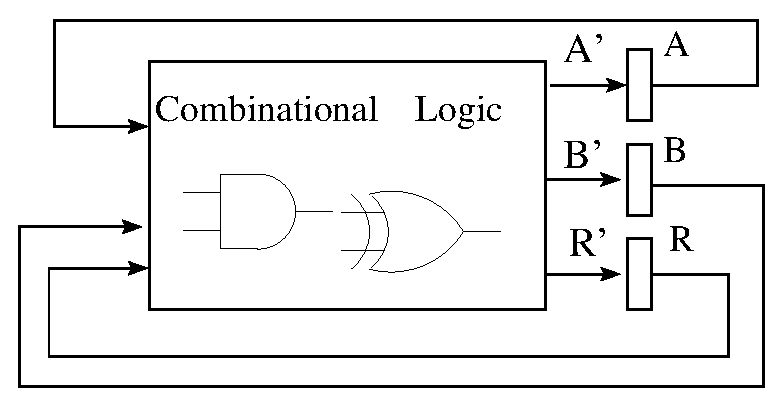
\includegraphics[width=5in]{newfig/gf_seq_model.eps}
\caption{A typical normal basis GF sequential circuit model. $A =
  (a_0,\dots,a_{k-1})$ and similarly $B, R$ are $k$-bit registers;
  $A', B', R'$ denote next-state inputs.}
\label{fig:sequential}}
\end{figure}

We follow  the sequential GF circuit model of
Figure \ref{fig:sequential}, with word-level variables $A, B, R$
denoting the {\it present states (PS)} and $A', B', R'$ denoting the {\it next
  states (NS)} of the machine; where $A = \sum_{i=0}^{k-1} a_i \beta^{2^i}$
for the PS variables and $A' = \sum_{i=0}^{k-1} a_i'
\beta^{2^i}$ for NS variables, and so on.  Variables $R\ (R')$ correspond to those that 
store the result, and $A, B\ (A', B')$ store input operands. E.g.,
for a GF multiplier, $A_{init}, B_{init}$ (and $R_{init} =
0$) are the initial values (operands) loaded into the registers,  and
$R = \Func(A_{init}, B_{init}) = A_{init} \times B_{init}$ is the final
result after $k$-cycles. Our approach aims to find this polynomial
representation for $R$.  

Each gate in the combinational logic is represented by a Boolean
polynomial. To 
this set of Boolean polynomials, we append the polynomials that define
the word-level to bit-level relations for PS and NS variables ($A =
\sum_{i=0}^{k-1} a_i \beta^{2^i}$). We denote this set of polynomials
as ideal $J = \langle 
f_1, \dots, f_s \rangle \subset \Fkk[x_1, \dots, x_d, R, R', A, A', B,
  B']$, where $x_1, \dots, x_d$ denote the bit-level (Boolean) variables
  of the circuit. The ideal of vanishing polynomials $J_0$ is also included, and
then the implicit FSM unrolling problem is setup for abstraction. 

The configurations of the flip-flops are the states of the
machine. Since the set of states is a finite set of points, we
can consider it as the variety of an ideal related to the circuit.
Moreover, since we are interested in
the function encoded by the state variables (over $k$-time
frames), we can project this variety on the word-level state
variables, starting from the initial state $A_{init}, B_{init}$.
Projection of varieties (geometry) corresponds to elimination ideals
(algebra), and can be analyzed via \Grobner bases. Therefore, we
employ a \Grobner basis computation with ATO: we use a {\it lex term
  order} with {\it bit-level variables} 
$>$ {\it word-level NS outputs} $>$ {\it word-level PS inputs}. This
allows to eliminate all the bit-level variables 
%(corresponding to the combinational logic and the state variables),
%so as to 
and derives a representation only in terms of words. 
Consequently, $k$-successive \Grobner basis computations implicitly
unroll the machine, and provide word-level algebraic $k$-cycle
abstraction for $R'$ as $R' = \Func(A_{init}, B_{init})$. 

Algorithm
\ref{alg:modified} describes our approach.  In the algorithm, $from_i$
and $to_i$ are polynomial ideals whose varieties are the valuations of
word-level variables $R, A, B$ and $R',A',B'$ in the $i$-th iteration;
and the notation ``$\setminus$'' signifies that the $NS$ in iteration
$(i)$ becomes the $PS$ in iteration $(i+1)$. Line 5 computes the Gr\"obner 
basis with the abstraction term order.  Line 6 computes the elimination 
ideal, eliminating the bit-level variables and representing the set of 
reachable states up to iteration $i$ in terms of the elimination ideal. 
These computations are analogous to those of image computations performed in 
the FSM reachability algorithm (given in Chapter \ref{ch:reacha}).

In the practice of sequential GF multiplier verification, the combinational 
logic actually implements function not only related to current operands $A$ and $B$,
but also involved with PS variable (i.e. temporary product) $R$. Which can be 
obtained using the abstraction:
$$R' = \Func(A,B,R)$$

Using ATO, if we put $R$ ahead of $R',A,B$ in term ordering, $R$ is thus eliminated
and the result in single iteration will be $R' = \Func(A,B)$. NS operands 
$A'$ and $B'$ are right-cyclic shift of $A$ and $B$, which can be directly written.
If initial values $A_{init}, B_{init}$ are treated as parameters, the NS ideal 
contains polynomials with $A', B'$ and $R' = \Func(A_{init},B_{init})$. This 
is also shown in the following example.


\begin{Example}[Functional verification of 5-bit RH-SMPO]
\label{ex:RHSMPO}
Figure \ref{fig:5bitRH} shows the detailed structure of a 5-bit RH-SMPO. The transition function for
operands $A,B$ is doing cyclic shift, while transition function for $R$ has to be computed through Gr\"obner basis
abstraction approach. Following ideal $J_{ckt}$ from line 5 in Algorithm \ref{alg:modified} is the ideal for 
all gates in combinational logic block and definition of word-level variables.
$$J_{ckt} = \langle f_1,f_2,\dots,f_{19}\rangle$$

\begin{eqnarray*}
 \left. 
\begin{aligned}
d_0+a_4b_4, c_1+a_0+a_4, c_2+b_0+b_4, d_1+c_1c_2, c_3+a_1a_4\\
c_4+b_1b_4, d_2+c_3c_4, e_0+d_0+d_1, e_3+d_1+d_2, e_4+d_2 \\
R_0+r_4+e_0, R_1+r_0, R_2+r_1, R_3+r_2+e_3, R_4+r_3+e_4
\end{aligned}\right\} ~~~\{f_1\dots f_{15}\}\\
 \left.
\begin{aligned}
 A+a_0\alpha^5+a_1\alpha^{10}+a_2\alpha^{20}+a_3\alpha^9+a_4\alpha^{18}\\
		  B+b_0\alpha^5+b_1\alpha^{10}+b_2\alpha^{20}+b_3\alpha^9+b_4\alpha^{18}\\
		  R'+r_0'\alpha^5+r_1'\alpha^{10}+r_2'\alpha^{20}+r_3'\alpha^9+r_4'\alpha^{18}\\
		  R+R_0\alpha^5+R_1\alpha^{10}+R_2\alpha^{20}+R_3\alpha^9+R_4\alpha^{18}
		 \end{aligned}\right\} ~~~\{f_{16}\dots f_{19}\}
\end{eqnarray*}

In our implementation here, since we only focus on the output variable $R$, evaluations of intermediate input 
operands $A, B$ are replaced by evaluations with parameters $A_{init},B_{init}$. 
Thus polynomials describing $A$ and $B$ ($f_{16}$ and $f_{17}$) can be removed from $J_{ckt}$, and $R$ is directly
evaluated by initial operands $A_{init}$ and $B_{init}$. Those two parameters are associated with PS bit-level inputs
$a_0,a_1,\dots,a_4$ and $b_0,b_1,\dots,b_4$ by polynomials given in $from^i$.

According to line 5 of Algorithm \ref{alg:modified}, we merge $J_{ckt}$, $J_0$ and $from^i$, then compute its
Gr\"obner basis with abstraction term order. 
Concretely, in the first iteration $from^0$ contains three generators. The first one describes PS variable $R$ --
temporary (or initial, in first iteration) product, which equals to 0 according to the mechanism of sequential 
GF multiplier. The polynomial is written as 
$$R$$
The other two polynomials describes PS variable $A,B$ -- current multiplication operands, and we write them 
in parameters $A_{init}, B_{init}$. Since this is the first iteration, they have the same form with $f_{16}$ and $f_{17}$:
\begin{align*}
& A_{init}+a_0\alpha^5+a_1\alpha^{10}+a_2\alpha^{20}+a_3\alpha^9+a_4\alpha^{18} \\
& B_{init}+b_0\alpha^5+b_1\alpha^{10}+b_2\alpha^{20}+b_3\alpha^9+b_4\alpha^{18}
\end{align*}
After computing the Gr\"obner basis of $J_{ckt}+J_0+from^0$ using ATO 
$$\text{all other bit-level variables} > R > \{R',A_{init},B_{init}\}$$
there is a polynomial in form of $R'+\Func(A_{init},B_{init})$,
which should be included by $to^{i+1}$. $to^{i+1}$ also exclude next state variable $A'$ and $B'$, instead we 
redefine $A_{init}$ and $B_{init}$ using next state bit-level variables $\{a_i', b_j'\}$. Next state Bit-level variables
$a_i' = a_{i-1\pmod k}, b_j' = b_{j-1\pmod k}$ according to definition of cyclic shift.

Line 7 in Algorithm \ref{alg:modified} is implemented by replacing $R'$ with $R$, $\{a_i', b_j'\}$ with $\{a_i,b_j\}$.

All intermediate results for each clock cycle are listed below:
\begin{itemize}
\item Clock-cycle 1: ${\bf from^0} = \{R, A_{init}+a_0\alpha^5+a_1\alpha^{10}+a_2\alpha^{20}+a_3\alpha^9+a_4\alpha^{18},
B_{init}+b_0\alpha^5+b_1\alpha^{10}+b_2\alpha^{20}+b_3\alpha^9+b_4\alpha^{18}\}$, \\
	${\bf to^1} = \{R'+(\alpha^4+\alpha^3+1) A_{init}^{16} B_{init}^{16}+(\alpha^4+\alpha^2) A_{init}^{16} B_{init}^4+(\alpha^3+1) A_{init}^{16} B_{init}^2+(\alpha^4+\alpha^3+1) A_{init}^{16} B_{init}+(\alpha^4+\alpha^3+\alpha^2+1) A_{init}^8 B_{init}^8+(\alpha^4+\alpha^3+\alpha+1) A_{init}^8 B_{init}^4+(\alpha^3+\alpha+1) A_{init}^8 B_{init}^2+(\alpha^4+\alpha^2) A_{init}^8 B_{init}+(\alpha^4+\alpha^2) A_{init}^4 B_{init}^{16}+(\alpha^4+\alpha^3+\alpha+1) A_{init}^4 B_{init}^8+(\alpha^2) A_{init}^4 B_{init}^4+(\alpha^3+\alpha^2+\alpha+1) A_{init}^4 B_{init}^2+(\alpha^4+\alpha^3+\alpha+1) A_{init}^4 B_{init}+(\alpha^3+1) A_{init}^2 B_{init}^{16}+(\alpha^3+\alpha+1) A_{init}^2 B_{init}^8+(\alpha^3+\alpha^2+\alpha+1) A_{init}^2 B_{init}^4+(\alpha^3+\alpha^2+\alpha) A_{init}^2 B_{init}^2+(\alpha^4+\alpha) A_{init}^2 B_{init}+(\alpha^4+\alpha^3+1) A_{init} B_{init}^{16}+(\alpha^4+\alpha^2) A_{init} B_{init}^8+(\alpha^4+\alpha^3+\alpha+1) A_{init} B_{init}^4+(\alpha^4+\alpha) A_{init} B_{init}^2+(\alpha^3+\alpha+1) A_{init} B_{init},
	A_{init}+a_4'\alpha^5+a_0'\alpha^{10}+a_1'\alpha^{20}+a_2'\alpha^9+a_3'\alpha^{18},
B_{init}+b_4'\alpha^5+b_0'\alpha^{10}+b_1'\alpha^{20}+b_2'\alpha^9+b_3'\alpha^{18}\}$
\item Clock-cycle 2: ${\bf from^1} = \{R+(\alpha^4+\alpha^3+1) A_{init}^{16} B_{init}^{16}+(\alpha^4+\alpha^2) A_{init}^{16} B_{init}^4+(\alpha^3+1) A_{init}^{16} B_{init}^2+(\alpha^4+\alpha^3+1) A_{init}^{16} B_{init}+(\alpha^4+\alpha^3+\alpha^2+1) A_{init}^8 B_{init}^8+(\alpha^4+\alpha^3+\alpha+1) A_{init}^8 B_{init}^4+(\alpha^3+\alpha+1) A_{init}^8 B_{init}^2+(\alpha^4+\alpha^2) A_{init}^8 B_{init}+(\alpha^4+\alpha^2) A_{init}^4 B_{init}^{16}+(\alpha^4+\alpha^3+\alpha+1) A_{init}^4 B_{init}^8+(\alpha^2) A_{init}^4 B_{init}^4+(\alpha^3+\alpha^2+\alpha+1) A_{init}^4 B_{init}^2+(\alpha^4+\alpha^3+\alpha+1) A_{init}^4 B_{init}+(\alpha^3+1) A_{init}^2 B_{init}^{16}+(\alpha^3+\alpha+1) A_{init}^2 B_{init}^8+(\alpha^3+\alpha^2+\alpha+1) A_{init}^2 B_{init}^4+(\alpha^3+\alpha^2+\alpha) A_{init}^2 B_{init}^2+(\alpha^4+\alpha) A_{init}^2 B_{init}+(\alpha^4+\alpha^3+1) A_{init} B_{init}^{16}+(\alpha^4+\alpha^2) A_{init} B_{init}^8+(\alpha^4+\alpha^3+\alpha+1) A_{init} B_{init}^4+(\alpha^4+\alpha) A_{init} B_{init}^2+(\alpha^3+\alpha+1) A_{init} B_{init},
	A_{init}+a_4\alpha^5+a_0\alpha^{10}+a_1\alpha^{20}+a_2\alpha^9+a_3\alpha^{18},
B_{init}+b_4\alpha^5+b_0\alpha^{10}+b_1\alpha^{20}+b_2\alpha^9+b_3\alpha^{18}\}$, \\
${\bf to^2} = \{R'+(\alpha^3+\alpha+1) A_{init}^{16} B_{init}^{16}+(\alpha^4+\alpha^3+1) A_{init}^{16} B_{init}^8+(\alpha^2) A_{init}^{16} B_{init}^4+(\alpha^3+1) A_{init}^{16} B_{init}^2+(\alpha^4+\alpha^3+1) A_{init}^8 B_{init}^{16}+(\alpha^4+\alpha^2) A_{init}^8 B_{init}^8+(\alpha^4) A_{init}^8 B_{init}^4+(\alpha^4+\alpha^3+1) A_{init}^8 B_{init}^2+(\alpha^3+1) A_{init}^8 B_{init}+(\alpha^2) A_{init}^4 B_{init}^{16}+(\alpha^4) A_{init}^4 B_{init}^8+(\alpha^4) A_{init}^4 B_{init}^4+(\alpha^4+\alpha^3+\alpha+1) A_{init}^4 B_{init}^2+(\alpha) A_{init}^4 B_{init}+(\alpha^3+1) A_{init}^2 B_{init}^{16}+(\alpha^4+\alpha^3+1) A_{init}^2 B_{init}^8+(\alpha^4+\alpha^3+\alpha+1) A_{init}^2 B_{init}^4+(\alpha^2) A_{init}^2 B_{init}^2+(\alpha^4+\alpha^3+\alpha^2+\alpha+1) A_{init}^2 B_{init}+(\alpha^3+1) A_{init} B_{init}^8+(\alpha) A_{init} B_{init}^4+(\alpha^4+\alpha^3+\alpha^2+\alpha+1) A_{init} B_{init}^2+(\alpha^4+\alpha^3+\alpha^2+\alpha+1) A_{init} B_{init},
A_{init}+a_3'\alpha^5+a_4'\alpha^{10}+a_0'\alpha^{20}+a_1'\alpha^9+a_2'\alpha^{18},
B_{init}+b_3'\alpha^5+b_4'\alpha^{10}+b_0'\alpha^{20}+b_1'\alpha^9+b_2'\alpha^{18}\}$
\item Clock-cycle 3: ${\bf from^2} = \{R+(\alpha^3+\alpha+1) A_{init}^{16} B_{init}^{16}+(\alpha^4+\alpha^3+1) A_{init}^{16} B_{init}^8+(\alpha^2) A_{init}^{16} B_{init}^4+(\alpha^3+1) A_{init}^{16} B_{init}^2+(\alpha^4+\alpha^3+1) A_{init}^8 B_{init}^{16}+(\alpha^4+\alpha^2) A_{init}^8 B_{init}^8+(\alpha^4) A_{init}^8 B_{init}^4+(\alpha^4+\alpha^3+1) A_{init}^8 B_{init}^2+(\alpha^3+1) A_{init}^8 B_{init}+(\alpha^2) A_{init}^4 B_{init}^{16}+(\alpha^4) A_{init}^4 B_{init}^8+(\alpha^4) A_{init}^4 B_{init}^4+(\alpha^4+\alpha^3+\alpha+1) A_{init}^4 B_{init}^2+(\alpha) A_{init}^4 B_{init}+(\alpha^3+1) A_{init}^2 B_{init}^{16}+(\alpha^4+\alpha^3+1) A_{init}^2 B_{init}^8+(\alpha^4+\alpha^3+\alpha+1) A_{init}^2 B_{init}^4+(\alpha^2) A_{init}^2 B_{init}^2+(\alpha^4+\alpha^3+\alpha^2+\alpha+1) A_{init}^2 B_{init}+(\alpha^3+1) A_{init} B_{init}^8+(\alpha) A_{init} B_{init}^4+(\alpha^4+\alpha^3+\alpha^2+\alpha+1) A_{init} B_{init}^2+(\alpha^4+\alpha^3+\alpha^2+\alpha+1) A_{init} B_{init},
A_{init}+a_3\alpha^5+a_4\alpha^{10}+a_0\alpha^{20}+a_1\alpha^9+a_2\alpha^{18},
B_{init}+b_3\alpha^5+b_4\alpha^{10}+b_0\alpha^{20}+b_1\alpha^9+b_2\alpha^{18}\}$, \\
${\bf to^3} = \{R'+(\alpha^4+\alpha^3+1) A_{init}^{16} B_{init}^{16}+(\alpha) A_{init}^{16} B_{init}^8+(\alpha^4+\alpha^3+\alpha^2+1) A_{init}^{16} B_{init}^4+(\alpha^4+\alpha^3+\alpha^2+\alpha+1) A_{init}^{16} B_{init}^2+(\alpha^4+\alpha^3+\alpha^2+1) A_{init}^{16} B_{init}+(\alpha) A_{init}^8 B_{init}^{16}+(\alpha+1) A_{init}^8 B_{init}^8+(\alpha^4) A_{init}^8 B_{init}^4+(\alpha^3+\alpha^2+1) A_{init}^8 B_{init}^2+(\alpha^4+\alpha^3+\alpha+1) A_{init}^8 B_{init}+(\alpha^4+\alpha^3+\alpha^2+1) A_{init}^4 B_{init}^{16}+(\alpha^4) A_{init}^4 B_{init}^8+(\alpha^4+\alpha^3+\alpha+1) A_{init}^4 B_{init}^4+(\alpha^3+\alpha+1) A_{init}^4 B_{init}^2+(\alpha^4+\alpha^3+\alpha^2+\alpha+1) A_{init}^4 B_{init}+(\alpha^4+\alpha^3+\alpha^2+\alpha+1) A_{init}^2 B_{init}^{16}+(\alpha^3+\alpha^2+1) A_{init}^2 B_{init}^8+(\alpha^3+\alpha+1) A_{init}^2 B_{init}^4+(\alpha^3+\alpha+1) A_{init}^2 B_{init}^2+(\alpha^4+\alpha^3+\alpha^2+1) A_{init} B_{init}^{16}+(\alpha^4+\alpha^3+\alpha+1) A_{init} B_{init}^8+(\alpha^4+\alpha^3+\alpha^2+\alpha+1) A_{init} B_{init}^4+(\alpha^4+\alpha) A_{init} B_{init},
A_{init}+a_2'\alpha^5+a_3'\alpha^{10}+a_4'\alpha^{20}+a_0'\alpha^9+a_1'\alpha^{18},
B_{init}+b_2'\alpha^5+b_3'\alpha^{10}+b_4'\alpha^{20}+b_0'\alpha^9+b_1'\alpha^{18}\}$
\item Clock-cycle 4: ${\bf from^3} = \{R+(\alpha^4+\alpha^3+1) A_{init}^{16} B_{init}^{16}+(\alpha) A_{init}^{16} B_{init}^8+(\alpha^4+\alpha^3+\alpha^2+1) A_{init}^{16} B_{init}^4+(\alpha^4+\alpha^3+\alpha^2+\alpha+1) A_{init}^{16} B_{init}^2+(\alpha^4+\alpha^3+\alpha^2+1) A_{init}^{16} B_{init}+(\alpha) A_{init}^8 B_{init}^{16}+(\alpha+1) A_{init}^8 B_{init}^8+(\alpha^4) A_{init}^8 B_{init}^4+(\alpha^3+\alpha^2+1) A_{init}^8 B_{init}^2+(\alpha^4+\alpha^3+\alpha+1) A_{init}^8 B_{init}+(\alpha^4+\alpha^3+\alpha^2+1) A_{init}^4 B_{init}^{16}+(\alpha^4) A_{init}^4 B_{init}^8+(\alpha^4+\alpha^3+\alpha+1) A_{init}^4 B_{init}^4+(\alpha^3+\alpha+1) A_{init}^4 B_{init}^2+(\alpha^4+\alpha^3+\alpha^2+\alpha+1) A_{init}^4 B_{init}+(\alpha^4+\alpha^3+\alpha^2+\alpha+1) A_{init}^2 B_{init}^{16}+(\alpha^3+\alpha^2+1) A_{init}^2 B_{init}^8+(\alpha^3+\alpha+1) A_{init}^2 B_{init}^4+(\alpha^3+\alpha+1) A_{init}^2 B_{init}^2+(\alpha^4+\alpha^3+\alpha^2+1) A_{init} B_{init}^{16}+(\alpha^4+\alpha^3+\alpha+1) A_{init} B_{init}^8+(\alpha^4+\alpha^3+\alpha^2+\alpha+1) A_{init} B_{init}^4+(\alpha^4+\alpha) A_{init} B_{init},
A_{init}+a_2\alpha^5+a_3\alpha^{10}+a_4\alpha^{20}+a_0\alpha^9+a_1\alpha^{18},
B_{init}+b_2\alpha^5+b_3\alpha^{10}+b_4\alpha^{20}+b_0\alpha^9+b_1\alpha^{18}\}$, \\
${\bf to^4} = \{R'+(\alpha^3+\alpha+1) A_{init}^{16} B_{init}^{16}+(\alpha^4+\alpha^3+\alpha^2+\alpha+1) A_{init}^{16} B_{init}^8+(\alpha^4+\alpha) A_{init}^{16} B_{init}^4+(\alpha^3+1) A_{init}^{16} B_{init}^2+(\alpha^3+\alpha+1) A_{init}^{16} B_{init}+(\alpha^4+\alpha^3+\alpha^2+\alpha+1) A_{init}^8 B_{init}^{16}+(\alpha^3+1) A_{init}^8 B_{init}^8+(\alpha^4+\alpha^2+\alpha) A_{init}^8 B_{init}^4+(\alpha^2+\alpha) A_{init}^8 B_{init}^2+(\alpha^3+\alpha^2+1) A_{init}^8 B_{init}+(\alpha^4+\alpha) A_{init}^4 B_{init}^{16}+(\alpha^4+\alpha^2+\alpha) A_{init}^4 B_{init}^8+(\alpha^4+\alpha^2+\alpha) A_{init}^4 B_{init}^4+(\alpha^2+\alpha) A_{init}^4 B_{init}+(\alpha^3+1) A_{init}^2 B_{init}^{16}+(\alpha^2+\alpha) A_{init}^2 B_{init}^8+(\alpha^4+\alpha^2) A_{init}^2 B_{init}^2+(\alpha^3+\alpha^2+1) A_{init}^2 B_{init}+(\alpha^3+\alpha+1) A_{init} B_{init}^{16}+(\alpha^3+\alpha^2+1) A_{init} B_{init}^8+(\alpha^2+\alpha) A_{init} B_{init}^4+(\alpha^3+\alpha^2+1) A_{init} B_{init}^2+(\alpha) A_{init} B_{init},
A_{init}+a_1'\alpha^5+a_2'\alpha^{10}+a_3'\alpha^{20}+a_4'\alpha^9+a_0'\alpha^{18},
B_{init}+b_1'\alpha^5+b_2'\alpha^{10}+b_3'\alpha^{20}+b_4'\alpha^9+b_0'\alpha^{18}\}$
\item Clock-cycle 5: ${\bf from^4} = \{R+(\alpha^3+\alpha+1) A_{init}^{16} B_{init}^{16}+(\alpha^4+\alpha^3+\alpha^2+\alpha+1) A_{init}^{16} B_{init}^8+(\alpha^4+\alpha) A_{init}^{16} B_{init}^4+(\alpha^3+1) A_{init}^{16} B_{init}^2+(\alpha^3+\alpha+1) A_{init}^{16} B_{init}+(\alpha^4+\alpha^3+\alpha^2+\alpha+1) A_{init}^8 B_{init}^{16}+(\alpha^3+1) A_{init}^8 B_{init}^8+(\alpha^4+\alpha^2+\alpha) A_{init}^8 B_{init}^4+(\alpha^2+\alpha) A_{init}^8 B_{init}^2+(\alpha^3+\alpha^2+1) A_{init}^8 B_{init}+(\alpha^4+\alpha) A_{init}^4 B_{init}^{16}+(\alpha^4+\alpha^2+\alpha) A_{init}^4 B_{init}^8+(\alpha^4+\alpha^2+\alpha) A_{init}^4 B_{init}^4+(\alpha^2+\alpha) A_{init}^4 B_{init}+(\alpha^3+1) A_{init}^2 B_{init}^{16}+(\alpha^2+\alpha) A_{init}^2 B_{init}^8+(\alpha^4+\alpha^2) A_{init}^2 B_{init}^2+(\alpha^3+\alpha^2+1) A_{init}^2 B_{init}+(\alpha^3+\alpha+1) A_{init} B_{init}^{16}+(\alpha^3+\alpha^2+1) A_{init} B_{init}^8+(\alpha^2+\alpha) A_{init} B_{init}^4+(\alpha^3+\alpha^2+1) A_{init} B_{init}^2+(\alpha) A_{init} B_{init},
A_{init}+a_1\alpha^5+a_2\alpha^{10}+a_3\alpha^{20}+a_4\alpha^9+a_0\alpha^{18},
B_{init}+b_1\alpha^5+b_2\alpha^{10}+b_3\alpha^{20}+b_4\alpha^9+b_0\alpha^{18}\}$, \\
${\bf to^5} = \{{\bf R'+A_{init}B_{init}},
A_{init}+a_0'\alpha^5+a_1'\alpha^{10}+a_2'\alpha^{20}+a_3'\alpha^9+a_4'\alpha^{18},
B_{init}+b_0'\alpha^5+b_1'\alpha^{10}+b_2'\alpha^{20}+b_3'\alpha^9+b_4'\alpha^{18}\}$
\end{itemize}
The algorithm returns
$$from^5(R_{final}) = R_{final}+A_{init} B_{init}$$
which is the function of the multiplier: $R_{final} = A_{init}\cdot B_{init}$
\end{Example}

\subsection{Overcome Computational Complexity using RATO}
% although commented, but I insist refer to previous chapter
% TODO experiment on naive slimgb on SMPO
We implement Algorithm \ref{alg:modified} in \textsc{Singular}, with the same setup and environment 
with the experiment in Section \ref{sec:exp_reacha}. The result on verifying Agnew's SMPO is shown 
in following table:

\begin{table}[H]
\label{tab:slimgb}
	\begin{center}
	    \caption{(Dummy)Runtime of Gr\"obner Basis Computation of Mastrovito Multipliers in Singular using ATO $>$.}\label{tab:ATO}
	    \begin{tabular}{|c|c||c|} 
	        \hline
		Word Size ($k$) & Number of Polynomials ($d$) & Computation Time (minutes)   \\
		\hline
	        $16$	&  $1,871$  & $2.4$ \\
		$24$	&  $3,135$  & $12$  \\
	        $32$	&  $5,549$  & $22.6$ \\
	        $40$	&  $8,587$  & $266$ \\
		$48$	& $12,327$  & NA (Out of Memory) \\
	        \hline
	    \end{tabular}
	\end{center} 
\end{table}

It indicates that our approach based on ATO cannot verify sequential GF multiplier with size larger than 40(dummy).
Similar to our improvements in Section \ref{sec:improve}, RATO \cite{TimDAC} is also available to 
accelerate the GB computation here. More specifically, we obviate the GB computation by turning the Buchberger's algorithm 
into a single-step multivariate polynomial division.

\begin{itemize}
\item First, a set of polynomials is constructed by polynomials translated from each logic gates, and they generate 
ideal $J_{gates}$. Similarly, ideal $J_{W-B}$ is generated by polynomials representing the word-bit correspondences.
They are merged as an ideal describing the combinational logic of the circuit: $J_{ckt} = J_{gates} + J_{W-B}$.
\item Second, we impose RATO on ideal $J_{ckt}$: all bit-level variables are sorted using reverse topological order
in circuit structure, followed by word-level NS output (e.g. $R'$ in Figure \ref{fig:sequential}), 
then word-level PS inputs (e.g. $A,B,R$ in Figure \ref{fig:sequential}).
\item When computing the Gr\"obner basis of $J_{ckt}+J_0$ (adding vanishing polynomials), because of 
RATO, there only exist one pair of polynomials $(f_w,f_g)$ such that $LCM(lm(f_w),lm(f_g)) \neq lm(f_w)\cdot lm(f_g)$.
\item Then we only need to compute the S-poly for $(f_w,f_g)$, the reduce the S-poly by $J_{ckt}+J_0$.
\end{itemize}

% first, in ideal generated by
% gates information polynomials and word-level variable definition polynomials, find the unique pair of polynomial
% generators with leading monomials not relatively prime to each other; then, compute their specification polynomial
% using definition 
% $$Spoly(f_w,f_g) = \frac{LCM}{lt(f_w)}\cdot f_w - \frac{LCM}{lt(f_g)}\cdot f_g$$
% where $LCM$ is least common multiple of $lm(f_w)$ and $lm(f_g)$, and $lt$ denotes the leading term;
% last, reduce $Spoly$ with ideal $J_{ckt}+J_0$, 
After executing the reduction, the remainder only contains a limited number of variables. It can be further 
transformed to a canonical polynomial
function of the circuit. We illustrate the whole improved procedure by applying RATO on 
5-bit RH-SMPO described in Example \ref{ex:RHSMPO} and Figure \ref{fig:5bitRH}.

\begin{Example}
\label{ex:newRATO}
From the circuit topological structure in Figure \ref{fig:5bitRH}, the term order under RATO is:
\begin{align}
&\{r_0',r_1',r_2',r_3',r_4'\}>\{r_0,r_1,r_2,r_3,r_4\}\nonumber\\
&>\{e_0,e_3,e_4\},\{d_0,d_1,d_2\},\{c_1,c_2,c_3,c_4\}\nonumber\\
&>\{a_0,a_1,a_2,a_3,a_4,b_0,b_1,b_2,b_3,b_4\}>R'>R>\{A,B\}\nonumber
\end{align}
The variables in braces are at the same topological level, they are arranged in LEX order. 
We search among all generators of $J_{ckt}$ from Example \ref{ex:RHSMPO} using RATO, 
and find a pair of polynomials whose leading 
monomials are not relatively prime:
$(f_w,f_g), f_w = r_0'+r_4+e_0, f_g =r_0'\alpha^5+r_1'\alpha^{10}+r_2'\alpha^{20}+r_3'\alpha^9+r_4'\alpha^{18} + R'$.
We calculate $Spoly$ can reduce it by $J_{ckt}+J_0$:
\begin{align}
&Spoly(f_w,f_g) \xrightarrow{J_{ckt}+J_0}_{+}\nonumber\\
&(\alpha^3+\alpha^2+\alpha) r_1+(\alpha^4+\alpha^3+\alpha^2) r_2+(\alpha^2+\alpha) r_3+(\alpha) r_4\nonumber\\
&+(\alpha^3+\alpha^2) a_1 b_1+(\alpha^4+\alpha^3+\alpha^2+\alpha) a_1 b_2+(\alpha^2+\alpha) a_1 b_3\nonumber\\
&+(\alpha^2+1) a_1 b_4+(\alpha^4+1) a_1 B+(\alpha^4+\alpha) a_2 b_1+(\alpha^4+\alpha^3+\alpha) a_2 b_2\nonumber\\
&+(\alpha^3+1) a_2 b_3+(\alpha^3+\alpha^2+1) a_2 b_4+(\alpha^3+\alpha^2) a_2 B+(\alpha^2+\alpha) a_3 b_1\nonumber\\
&+(\alpha^3+1) a_3 b_2+(\alpha+1) a_3 b_3+(\alpha^4+\alpha^2+\alpha) a_3 b_4\nonumber\\
&+(\alpha^4+\alpha^3+\alpha) a_3 B+(\alpha^3+1) a_4 b_1+a_4 b_2+(\alpha^4+\alpha^2+\alpha) a_4 b_3\nonumber\\
&+(\alpha^4+\alpha^3+1) a_4 b_4+(\alpha^2+\alpha) a_4 B+(\alpha^4+1) b_1 A+(\alpha^3+\alpha^2) b_2 A\nonumber\\
&+(\alpha^4+\alpha^3+\alpha) b_3 A+(\alpha^2+\alpha) b_4 A+(\alpha^4+\alpha^2+\alpha+1) R'+R+A B\nonumber
\end{align}
\end{Example}
Above example indicates that RATO based abstraction on 5-bit RH-SMPO will result a remainder containing both
bit-level variables and word-level variables. Moreover, the number of variables is still large such that
Gr\"obner basis computation will be inefficient.

Since the remainder from \emph{Spoly} reduction contains some bit-level variables, our objective is to compute
a polynomial that contains only word-level variables (such as $R'+\mathcal{F}(A,B)$). One possible solution to
this problem is to replace bit-level variables by equivalent polynomials that only contain word-level
variables, e.g. $a_i = \mathcal{G}(A), r_j = \mathcal{H}(R)$. In this section a Gaussian-elimination
approach is introduced to compute corresponding $\mathcal{G}(A),\mathcal{H}(R)$ efficiently.

\begin{Example}
\label{ex:BLVS}
{\bf Objective}:\ Compute polynomial $a_i + \mathcal{G}_i(A)$ from $f_0 = a_0\alpha^5+a_1\alpha^{10}+a_2\alpha^{20}+a_3\alpha^9+a_4\alpha^{18}+A
 = g_0 + A$.

First, compute $f_0^2= a_0\alpha^{10}+a_1\alpha^{20}+a_2\alpha^{9}+a_3\alpha^{18}+a_4\alpha^{5}+A^2 = g_0^2 + A^2$;
then $f_0^4, f_0^8, f_0^{16}$. By repeating squaring we get a system of equations:
\begin{displaymath}
  \begin{cases}
  f_0  &=\ \  0\\
  f_0^2 & =\ \  0\\
  f_0^4  &=\ \  0\\
  f_0^8  &=\ \  0\\
  f_0^{16} & =\ \ 0
  \end{cases}
\Longleftrightarrow\ \
\begin{cases}
  g_0 & =\ \  A\\
  g_0^2 & =\ \  A^2\\
  g_0^4 & =\ \  A^4\\
  g_0^8 & =\ \  A^8\\
  g_0^{16} & =\ \  A^{16}
  \end{cases}
\end{displaymath}
Following is the coefficients matrix form of this system of equations:
\begin{displaymath}
\begin{pmatrix}
\alpha^5 & \alpha^{10} & \alpha^{20} & \alpha^9 & \alpha^{18} \\
\alpha^{10} & \alpha^{20} & \alpha^9 & \alpha^{18} & \alpha^5 \\
\alpha^{20} & \alpha^9 & \alpha^{18} & \alpha^5 & \alpha^{10} \\
\alpha^9 & \alpha^{18} & \alpha^5 & \alpha^{10} & \alpha^{20} \\
\alpha^{18} & \alpha^5 & \alpha^{10} & \alpha^{20} & \alpha^9 
\end{pmatrix}
\begin{pmatrix}
a_0\\
a_1\\
a_2\\
a_3\\
a_4
\end{pmatrix}
=
\begin{pmatrix}
A\\
A^2\\
A^4\\
A^8\\
A^{16}
\end{pmatrix}
\end{displaymath}

Then we use Gaussian elimination on coefficients matrix 
% \begin{align}
% Row\ 2 =& Row\ 1\times \alpha^5 + Row\ 2: \nonumber\\
% &a_1+(\alpha)a_2+(\alpha^4+\alpha^2)a_3+(\alpha^3+\alpha^2)a_4\nonumber\\
% =&(\alpha^4+\alpha^3+\alpha^2+1)A^2+(\alpha^2+\alpha)A\nonumber
% \end{align}
to recursively eliminate $a_1$ from third row, $a_2$ from fourth row, etc. The final solution to this system of
equations is
%\begin{displaymath}
%\{g_i\ | \ g_i: a_i + \mathcal{G}_i(A)\}
%\end{displaymath}
%\end{Example}
\begin{displaymath}
\left\{
  \begin{array}{lcl}
  a_0 & = & (\alpha+1)A^{16}+(\alpha^4+\alpha^3+\alpha)A^8+(\alpha^3+\alpha^2)A^4\\&&+(\alpha^4+1)A^2+(\alpha^2+1)A\\
  a_1 & = & (\alpha^2+1)A^{16}+(\alpha+1)A^8+(\alpha^4+\alpha^3+\alpha)A^4\\&&+(\alpha^3+\alpha^2)A^2+(\alpha^4+1)A\\
  a_2 & = & (\alpha^4+1)A^{16}+(\alpha^2+1)A^8+(\alpha+1)A^4\\&&+(\alpha^4+\alpha^3+\alpha)A^2+(\alpha^3+\alpha^2)A\\
  a_3 & = & (\alpha^3+\alpha^2)A^{16}+(\alpha^4+1)A^8+(\alpha^2+1)A^4\\&&+(\alpha+1)A^2+(\alpha^4+\alpha^3+\alpha)A\\
  a_4 & = & (\alpha^4+\alpha^3+\alpha)A^{16}+(\alpha^3+\alpha^2)A^8+(\alpha^4+1)A^4\\&&+(\alpha^2+1)A^2+(\alpha+1)A
  \end{array} \right.
\end{displaymath}
\end{Example}
Similarly we can compute equivalent polynomials $\mathcal{H}_i(R)$ for $r_i$ and $\mathcal{T}_j(B)$ for $b_j$, respectively.
Using those polynomial equations, it is sufficient to translate all bit-level inputs in the remainder polynomial
because of following lemma:
\begin{Proposition}
\label{lem:bitlevelremainder}
Remainder of S-poly reduction will only contain primary inputs (bit-level) and word-level output; furthermore, there will be one and
only one term containing word-level output whose monomial is word-level output itself rather than higher order form.
\end{Proposition}

\begin{Proof}
First proposition is easy to prove by contradiction: assume there exists an intermediate bit-level variable $v$ in the remainder,
then this remainder must be divided further by a polynomial with leading term $v$. 
Since the remainder cannot be divided by any other polynomials in $J_{ckt}$, the assumption does not hold.

Second part, the candidate pair of polynomials only have one term of
single word-level output variable (say it is $R$) and this term is the last term under RATO, which means there is only one term with
$R$ in Spoly. Meanwhile in other polynomials from $J_{ckt}+J_0$ there is no such term containing $R$, so this term will be
kept to remainder $r$, with exponent equals to 1.
\end{Proof}

By replacing all bit-level variables by corresponding word-level variable polynomials, we transform the remainder
of $Spoly$ reduction to the form of $R'+R+\mathcal F'(A,B)$. Note $R$ is present state notion of output, which
equals to initial value $R=0$ in first clock cycle, or value of $R'$ from last clock cycle. By substituting
$R$ with its corresponding value ($0$ or a polynomial only about $A$ and $B$), we get the desired polynomial function
$R'+\mathcal F(A,B)$.

\subsection{Solving a Linear System for Bit-to-Word Substitution}
In Example \ref{ex:BLVS} we use a Gaussian-elimination method to solve the system of polynomial
equations. We describe another formal method to solve following system of equations
\begin{align}
\label{eqn:betamat}
\begin{bmatrix}
S \\
S^2 \\
S^{2^2} \\
\vdots \\
S^{2^{k-1}}
\end{bmatrix}
&=
\begin{bmatrix}
\beta & \beta^{2} & \beta^{2^2} & \cdots & \beta^{2^{k-1}}\\
\beta^{2} & \beta^{2^2} & \beta^{2^3} & \cdots & \beta \\
\beta^{2^2} & \beta^{2^3} & \beta^{2^4} & \cdots & \beta^2\\
\vdots & \vdots & \vdots & \ddots & \vdots \\
\beta^{2^{k-1}} & \beta & \beta^2 & \cdots & \beta^{2^{k-2}}
\end{bmatrix}
\begin{bmatrix}
s_0\\
s_1\\
s_2\\
\vdots\\
s_{k-1}
\end{bmatrix}
\end{align}
Let ${\bf s}$ be a vector of $k$ unknowns $s_0,\dots,s_{k-1}$,
then Equation \ref{eqn:betamat} can be solved by using Cramer's rule:
\begin{equation}
\label{eqn:Cramer}
s_i = \frac{\Mi}{\M}, \ \ 0\leq i\leq k-1, \M \neq 0
\end{equation}
where ${\bf M_i}$ denotes a coefficient matrix replacing $i$-th column in ${\bf M}$ with
vector ${\bf S} = [S~~S^2~~\cdots~~S^{2^{k-1}}]^T$.

Notice that ${\bf M}$ is constructed by squaring a row and assigning it to next row,
therefore its determinant exhibits certain special properties:
\begin{Definition}
Let $\{\alpha_0,\alpha_1,\dots,\alpha_{k-1}\}$ be a set of $k$ elements of $\Fpk$. Then the determinant
\begin{align}
\det{M(\alpha_0,\dots,\alpha_{k-1})} &= 
\begin{vmatrix}
\alpha_0 & \alpha_1 & \cdots & \alpha_{k-1} \\
\alpha_0^p & \alpha_1^p & \cdots & \alpha_{k-1}^p \\
\vdots & \vdots & \ddots & \vdots \\
\alpha_0^{p^{k-1}} & \alpha_1^{p^{k-1}} & \cdots & \alpha_{k-1}^{p^{k-1}}
\end{vmatrix}
\end{align}
is called the {\bf Moore determinant} of set $\{\alpha_0,\dots,\alpha_{k-1}\}$.
\end{Definition}
Moore determinant can be written as an explicit expression
\begin{equation}
\label{eqn:Moore}
\det{M(\alpha_0,\dots,\alpha_{k-1})} = \alpha_0 \prod_{i=1}^{k-1}\left( \prod_{c_0,\dots,c_{i-1}\in \Fp} (\alpha_{i} - \sum_{j=0}^{i-1}c_j\alpha_j)\right)
\end{equation}
We use an example to help understanding the notations in Equation \ref{eqn:Moore}:
\begin{Example}
Let $\{\alpha_0,\alpha_1,\alpha_2\}$ be a set of elements of $\mathbb F_{2^3}$. Then
\begin{align}
\det{M(\alpha_0,\alpha_1,\alpha_2)} &= 
\begin{vmatrix}
\alpha_0 & \alpha_1 & \alpha_2 \\
\alpha_0^2 & \alpha_1^2 & \alpha_2^2 \\
\alpha_0^4 & \alpha_1^4 & \alpha_2^4
\end{vmatrix} \\ \nonumber
=& \alpha_0 \prod_{i=1}^{2} \prod_{c_0,\dots,c_{i-1}\in \mathbb F_2} (\alpha_{i} - \displaystyle\sum_{j=0}^{i-1}c_j\alpha_j)
\end{align}
First, let $i=1$,  we obtain $c_0\in \mathbb F_2$. When $c_0=0$, the product term equals to $\alpha_1$; when $c_0=1$ it equals to $(\alpha_1-\alpha_0)$.
Then let $i=2$, we obtain ${c_0,c_1}\in \mathbb F_2$, they can take value from $\{0,0\},\{0,1\},\{1,0\}$ and $\{1,1\}$.
We add 4 more product terms $\alpha_2,(\alpha_2-\alpha_1),(\alpha_2-\alpha_0),(\alpha_2-\alpha_0-\alpha_1)$, respectively.

Thus, the result is
\begin{equation}
\det{M(\alpha_0,\alpha_1,\alpha_2)} = \alpha_0\alpha_1(\alpha_1-\alpha_0)\alpha_2(\alpha_2-\alpha_1)(\alpha_2-\alpha_0)(\alpha_2-\alpha_0-\alpha_1)
\end{equation}
\end{Example}
We discover through investigation that $\M$ has a special property when the set of elements forms a basis. The proof is given below:
\begin{Lemma}
\label{lemma:Moore}
Let $\{\alpha_0,\alpha_1,\dots,\alpha_{k-1}\}$ be a normal basis of $\Fpk$ over $\Fp$. Then
\begin{equation}
\det{M(\alpha_0,\alpha_1,\dots,\alpha_{k-1})} = 1
\end{equation}
\end{Lemma}
\begin{Proof}
According to the definition Equation \ref{eqn:Moore}, the Moore determinant consists of all possible linear combinations of 
$\{\alpha_0,\alpha_1,\dots,\alpha_{k-1}\}$ with coefficients over $\Fp$. If $\{\alpha_0,\alpha_1,\dots,\alpha_{k-1}\}$
is a (normal) basis, then all product terms are distinct and represents all elements in the field $\Fpk$. Since the product 
of all elements of a field equals to 1, the Moore determinant $\M=1$.
\end{Proof}

Applying Lemma \ref{lemma:Moore} to Equation \ref{eqn:Cramer} gives
\begin{equation}
s_i = \Mi,~~0\leq i\leq k-1
\end{equation}
where $\Mi$ can be easily computed using Laplace expansion method, with complexity $O(k!)$.

% However, we observe a fact that solution, if written as the inversion of matrix $M$, is a circulant matrix itself.
% We have following proposition:
% $$\dots$$
% Therefore, for a certain type of ONB, we can directly write down the inversion of corresponding matrix $M$
% as 
% $$\dots$$
% TODO Since our finding only works on type-II ONB, too complicated to explain, so omit

\subsection{The Overall Verification Approach}
Based on above concepts and improvements, the functional verification for sequential GF multiplier 
on word-level with $k$-bit input operands $A,B$ and $k$-bit output $R$ is described as follows:
\begin{enumerate}[{1)}]
\item Given a sequential GF multiplier $S$, with word-level $k$-bit inputs $A,B$ and output $R$.
\item Choose a primitive polynomial $P(x)$ of degree $k$ and construct $\Fkk$, and let $P(\alpha)=0$.
\item Perform a reverse-topological traversal of $S$ to derive RATO: LEX with $\{x_1>x_2>\cdots>x_d>R'>R>A>B\}$,
where $\{x_1,\dots,x_d\}$ are bit-level variables of $S$, $R'$ is the NS output value.
\item Derive the set of bit-level polynomials $\{f_1,\dots,f_s\}$ from each gate in $S$, and represent them 
using RATO. These polynomials are in the form $x_i+tail(f_i)$ where $x_i$ is the output of corresponding gate.
\item Compose the bit-level to word-level correspondences polynomials such as $r_0\beta+r_1\beta^2+\cdots+r_{k-1}\beta^{2^{k-1}}+R$.
Add them to set $\{f_1,\dots,f_s\}$ and generate ideal $J_{ckt}$. Compose the ideal of vanishing polynomials
$J_0 = \langle x_i^2+x_i, \dots, R^{2^k}+R,\dots\rangle$.
\item Select the only critical pair $(f_w,f_g)$ that does not have relatively prime leading terms. Compute
$Spoly(f_w,f_g) \xrightarrow{J_{ckt}+J_0}_{+}r$.
\item Construct matrices $M_0,\dots,M_{k-1}$, where $M_i$ is $M$ with the $i$-column replaced by vector 
$[R R^2 \cdots R^{2^{k-1}}]^T$, and $M$ is the reverse-circulant matrix generated by vector $(\beta,\beta^2,\dots,\beta^{2^{k-1}})$.
\item Symbolically compute the determinants $|M_i|$ to find set $F_R$, where $f_{R_i}:R_i+|M_i|$, for $0\leq i \leq k-1$.
Obtain $F_A, F_B$ from $F_R$ since they have the same form.
\item Compute $r \xrightarrow{F_A\cup F_B \cup F_R}_{+}r_w$, and iterate $r_w$ as $to^i$ in Algorithm \ref{alg:modified}.
{\bf Then $r_w$ after iteration $k$ is of the form $R'+\Func(A,B)$ and it is the unique, canonical word-level abstraction
of $S$ over $\Fkk$ after $k$ clock-cycles}.
\end{enumerate}

\section{Software Implementation of Implicit Unrolling Approach}
Our experiment on different size of SMPO designs is performed with both \textsc{Singular} \cite{DGPS}
symbolic algebra computation system and our customized toolset developed using C++.
The SMPO designs are given as gate-level netlists with registers, then translated to polynomials to compose
elimination ideal for Gr\"obner basis calculation. The experiment is conducted on desktop with
3.5GHz Intel $\text{Core}^\text{TM}$ i7 Quad-core CPU, 16 GB RAM and running 64-bit Linux OS.

The \textsc{Singular} tool can read in scripts written in its own format similar to ANSI-C. 
The input file format for our C++ tool is also designed to compatible with \text{Singular} 
ring and polynomial definitions. For SMPO experiments, the main 
loop of our script file performs the same function as Algorithm \ref{alg:modified} describes, while Gr\"obner basis
computation in main loop can be divided into 4 different function parts:

1) Pre-process:

This step is executed only once before main loop starts. The function of pre-process is to compute following system
of equations for bit-level inputs $a_0 \dots a_{k-1}$:
\begin{displaymath}
\left\{
  \begin{array}{ll}
  a_0 & = f_0(A)\\
  a_1 & = f_1(A)\\
  \vdots & \ \\
  a_{k-1} & = f_{k-1}(A)
  \end{array} \right.
\end{displaymath}
The methodology has been discussed in this chapter. For 5-bit SMPO example, we start from bit-word correspondence polynomial
\begin{displaymath}
A + a_0\alpha^5+a_1\alpha^{10}+a_2\alpha^{20}+a_3\alpha^9+a_4\alpha^{18}
\end{displaymath}
and the result is
\begin{displaymath}
\left\{
  \begin{array}{lcl}
  a_0 & = & (\alpha+1)A^{16}+(\alpha^4+\alpha^3+\alpha)A^8+(\alpha^3+\alpha^2)A^4\\&&+(\alpha^4+1)A^2+(\alpha^2+1)A\\
  a_1 & = & (\alpha^2+1)A^{16}+(\alpha+1)A^8+(\alpha^4+\alpha^3+\alpha)A^4\\&&+(\alpha^3+\alpha^2)A^2+(\alpha^4+1)A\\
  a_2 & = & (\alpha^4+1)A^{16}+(\alpha^2+1)A^8+(\alpha+1)A^4\\&&+(\alpha^4+\alpha^3+\alpha)A^2+(\alpha^3+\alpha^2)A\\
  a_3 & = & (\alpha^3+\alpha^2)A^{16}+(\alpha^4+1)A^8+(\alpha^2+1)A^4\\&&+(\alpha+1)A^2+(\alpha^4+\alpha^3+\alpha)A\\
  a_4 & = & (\alpha^4+\alpha^3+\alpha)A^{16}+(\alpha^3+\alpha^2)A^8+(\alpha^4+1)A^4\\&&+(\alpha^2+1)A^2+(\alpha+1)A
  \end{array} \right.
\end{displaymath}
By replacing bit-level variable $a_i$ with $b_i, r_i$ or $r_i'$, and word-level variable $A$ with $B, R, R'$ respectively,
we can directly get bit-word relation functions for another operand input, pseudo input and pseudo output.

One limitation to \textsc{Singular} tool is the degree of a term cannot exceed $2^{63}$, so when conducting experiments 
for SMPO circuits larger than
62 bits, we rewrite the degree using smaller integers (the feasibility of this rewriting can also be verified 
in following steps). Our C++ tool does not have data size limit, but it accumulates exponent when computing 
the power of a variable. Thus if the exponent is as large as $2^{63}$, its runtime is very long. As a 
result, our C++ tool also adopts and benefits from this rewriting technique.
Since the bit-to-word substitution procedure
only requires squaring of equations each time, the exponent of word $A$ can only be in the form $2^{i-1}$, i.e. 
$A^{2^0},A^{2^1},\dots,A^{2^{k-1}}$. To minimize the exponents presenting in both \textsc{Singular} and our tool, 
we rewrite exponent $2^{i-1}$ to exponent $i$, i.e.
$(A^{2^0},A^{2^1},\dots,A^{2^{k-1}}) \to (A, A^2, \dots, A^k)$. In this way result is rewritten to be
$$a_0 = (\alpha+1)A^5+(\alpha^4+\alpha^3+\alpha)A^4+(\alpha^3+\alpha^2)A^3+(\alpha^4+1)A^2+(\alpha^2+1)A$$
Thus the exponents do not exceed the \textsc{Singular} data size limit.

This step requires limited substitution operations, so although we use the naive Gaussian elimination
method (whose time complexity is $O(k^3)$), the time cost is trivial comparing to following steps. 
% For 33 bits experiment,
% pre-process execution time is 2.7 sec; while for 100 bits experiment time cost is 36 sec.

2) S-poly reduction:

First, S-poly is calculated based on RATO, then reduced with the ideal composed by circuit description polynomials ($J_{ckt}$).
For already finished experiments, naive reduction (multi-division) is adopted, and this step takes largest portion of total 
time consumption.

For SMPO experiments, reduced Spoly has following generic form (all coefficients are omitted):
$$redSpoly = R'+\Func(a_i,b_j,r_l,A,B,R) = \sum r_i + \sum a_ib_i + \sum a_iB + \sum b_iA + R' + R$$
From observation, there is no cross-product terms of bit-by-bit or bit-by-word variables from the same input/output
such as $a_ia_j, a_iA$, etc. Consider the necessary
condition of our trick, this property of reduced Spoly guarantees the word level variable can only exist in the form $A^{2^{i-1}}$,
after substituting bit-level variables with corresponding word-level variable.

3) Substitute bit-level variables in reduced S-poly, i.e. 
$$\Func(a_i,b_j,r_l,A,B,R) \xrightarrow{a_i+\mathcal{G}_i(A),b_j+\mathcal{G}_j(B),r_l+\mathcal{G}_l(R)} \mathcal{H}(A,B,R)$$

Use the result from pre-process, get rid of $r_i, a_i$ and $b_i$ through substitution. This step yields following polynomial (consider the trick we used):
\begin{equation}
\label{eqn:HABR}
R'+ \mathcal{H}(A,B,R) = R' + \sum R^i + \sum A^iB^j
\end{equation}
all coefficients omitted.

4) Substitute PS word-level variable $R$ with inputs $A$ and $B$, i.e. 
$$\Func(A,B,R) \xrightarrow{R+\Func'(A,B)} \Func(A,B)$$

In Equation \ref{eqn:HABR}, there are still terms containing $R$ in the ideal we want to compute Gr\"obner basis.
For PS variable $R$ we can use relation $R+\Func'(A,B)$, which is the last clock-cycle's output ($R'+\Func'(A,B)$) 
with only leading term replaced in step "$from^i\gets to^i$" in 
Algorithm \ref{alg:modified}. Basically this step has nothing different from the last one, however, the degree
of its terms are not actual degree because of the exponent rewriting technique. For example,
a power of $r$ -- $r^m$ is originally $r^{2^{m-1}}$. So if $R+\Func'(A,B)$ contains terms $A^iB^j$, the result 
after exponent rewriting
is $$(A^{2^{i-1}}B^{2^{j-1}})^{2^{m-1}} = A^{2^{((i+m-2)\bmod k)+1}}B^{2^{((j+m-2)\bmod k)+1}}$$
Thus the actual exponent for $A$ and $B$ in $(A^iB^j)^m$ should be $((i+m-2)\bmod k)+1$ and $((j+m-2)\bmod k)+1$, respectively.

Within one iteration, after finishing steps 2) to 4), the output should be intermediate multiplication result (temporary product) 
$R'+\Func(A,B)$. After $k$ iterations,
the output is $R+A\cdot B$ when SMPO circuit is bug-free.

% \subsection{Architecture in Customized C++ Toolset}
% what kind of package, what kind of data structure, what kind of algorithm we use (refer to preliminaries part)

\section{Experimental Results}
\label{sec:result}
% TODO revise repeated parts and references, add C++ results

We have implemented our approach within the \textsc{Singular} symbolic
algebra computation system [v. 3-1-6] \cite{DGPS} as well as C++/GCC. Using our
implementation, we have performed experiments to verify two SMPO
architectures --- Agnew-SMPO \cite{agnew1991implementation} and the
RH-SMPO \cite{RHmulti} --- over $\Fkk$, for various datapath/field
sizes. Bugs are also introduced into the SMPO designs by modifying a
few gates in the combinational logic block. Experiments using SAT-,
BDD-, and AIG-based solvers are also conducted and results are
compared against our approach.  Our experiments run on a desktop with
3.5GHz Intel $\text{Core}^\text{TM}$ i7 Quad-core CPU, 16 GB RAM and
64-bit Linux.   

{\it Evaluation of SAT/ABC/BDD based methods:} To verify circuit $S$
against the polynomial $\Func$, we unroll the SMPO over $k$ time-frames,
and construct a miter against a combinational implementation of $\Func$.
A (pre-verified) $\Fkk$ Mastrovito multiplier \cite{mastro:1989} is
used as the {\it spec} model. This miter is checked for SAT using the
\emph{Lingeling} \cite{biere2013lingeling} solver. We also experiment
with the Combinational Equivalence Checking (CEC) engine of the ABC
tool \cite{abc}, which uses AIG-based reductions to identify internal
AIG equivalences within the miter to efficiently solve
verification. The BDD-based VIS tool \cite{brayton1996vis} is also used
for equivalence check. The run-times for verification of (unrolled)
RH-SMPO against Mastrovito {\it   spec} are given in Table
\ref{tbl:equiv} -- which shows that the techniques fail beyond 23 bit
fields.  

\vspace{-0.1in}
\begin{table}[htb]
\centering
\caption{\small Run-time for verification of bug-free RH-SMPO circuits
  for SAT, ABC and BDD based methods. \emph{TO} = timeout 14 hrs}
\label{tbl:equiv}
\begin{tabular}{|c||c|c|c|c|} 
\hline
& \multicolumn{4}{|c|}{Word size of the operands $k$-bits}  \\
\hline
Solver & 11 & 18 & 23 & 33 \\
\hline
\hline
Lingeling & 593  & \emph{TO}  & \emph{TO}  & \emph{TO}\\
\hline
\hline
ABC & 6.24 & \emph{TO} & \emph{TO} & \emph{TO}\\
\hline
\hline
BDD & 0.1 & 11.7 & 1002.4 & \emph{TO}  \\
\hline
\end{tabular}
\label{table:satbdd}  
\end{table} 

CEC between unrolled RH-SMPO and Agnew-SMPO also suffers the same fate
(results omitted). In fact, both SMPO designs are based on slightly
different mathematical concepts and their computations in all
clock-cycles, except for the $k^{th}$ one, are also different. These
designs have no internal logical/structural equivalencies, and
verification with SAT/BDDs/ABC is infeasible. Their dissimilarity is
depicted in Table \ref{tbl:fraig}, where  $N_1$ depicts the number of
AIG nodes in the miter prior to {\it fraig\_sweep}, and the nodes
after {\it fraiging} are recorded as $N_2$; so $\frac{N_1-N_2}{N_1}$
reflects the proportion of equivalent nodes in original miter, which
emphasizes the (lack of) \emph{similarity} between two designs.  

\begin{table}[htb]
\centering
\caption{\small Similarity between RH-SMPO and Agnew's SMPO}
\label{tbl:fraig}
\begin{tabular}{|c||c|c|c|c|} 
\hline
Size $k$ & 11 & 18 & 23 & 33 \\
\hline
$N_1$ & 734  & 2011  & 3285  & 6723\\
\hline
$N_2$ & 529 & 1450 & 2347 & 4852\\
\hline
Similarity & $27.9\%$ & $27.9\%$ & $28.6\%$ & $27.8\%$  \\
\hline
\end{tabular}\label{table:similarity}  
\end{table} 

{\it Evaluation of Our Approach:} Our algorithm inputs the circuit
given in BLIF format, derives RATO, and constructs the polynomial
ideal from the logic gates and the register/data-word description.  We
perform one $Spoly$ reduction, followed by the bit-level to word-level 
substitution, in each clock cycle. After $k$ iterations, the final
result polynomial $R$ is compared against the spec polynomial. The
run-times for verifying bug-free and buggy RH-SMPO and Agnew-SMPO are
shown in Table \ref{tbl:exp1} and Table \ref{tbl:exp2}, respectively. 
We can verify, as well as catch bugs in, up to 100-bit
multipliers. Beyond 100-bit fields, our approach is infeasible --
mostly due to the fact that the intermediate 
abstraction polynomial $R$ is very dense and contains high-degree
terms, which can be infeasible to compute. However, it should be noted
that if we do not use the proposed bit-level to word-level
substitution, and compute reduced \Grobner bases with RATO, then our
approach does not scale beyond 33-bit datapaths. 

\begin{table}[htb]
\centering
\caption{\small Run-time (seconds) for verification of bug-free and
  buggy RH-SMPO using our approach} 
\label{tbl:exp1}  
\begin{tabular}{|c||c|c|c|c|c|c|} 
\hline
Operand size $k$ & 33 & 51 & 65 & 81 & 89 & 99\\
\hline
\#variables & 4785 & 11424 & 18265 & 28512 & 34354 & 42372\\
\hline
\#polynomials & 3630 & 8721 & 13910 & 21789 & 26255 & 32373\\
\hline
\#terms & 13629 & 32793 & 52845 & 82539 & 99591 & 122958\\
\hline
\hline
Runtime(bug-free) & 112.6 & 1129 & 5243 & 20724 & 36096 & 67021\\
\hline
Runtime(buggy) & 112.7 & 1129 & 5256 & 20684 & 36120 & 66929\\
\hline
\end{tabular}
%\begin{minipage}{8cm}
%\def\arraystretch{1.5}\tabcolsep 2pt
%% \begin{tabular}{|c||c|c|c|c|c|} 
%% \hline
%% Operand size $k$ & 33 & 51 & 65 & 81 & 89 \\
%% \hline
%% \#variables & 4785 & 11424 & 18265 & 28512 & 34354\\
%% \hline
%% \#polynomials & 3630 & 8721 & 13910 & 21789 & 26255\\
%% \hline
%% \#terms & 13629 & 32793 & 52845 & 82539 & 99591 \\
%% \hline
%% %\hline
%% Runtime(bug-free) & 112.6 & 1129 & 5243 & 20724 & 36096 \\
%% \hline
%% Runtime(buggy) & 112.7 & 1129 & 5256 & 20684 & 36120\\
%% \hline
%% \hline
%% \end{tabular}
%% %\end{minipage}
\end{table}

\begin{table}[hbt]
\centering
\caption{\small Run-time (seconds) for verification of
  bug-free and buggy Agnew's SMPO our approach}
\label{tbl:exp2}
\begin{tabular}{|c||c|c|c|c|c|} 
\hline
Operand size $k$ & 36 & 66 & 82 & 89 & 100 \\
\hline
\#variables & 6588 & 21978 & 33866 & 39872 & 50300\\
\hline
\#polynomials & 2700 & 8910 & 13694 & 16109 & 20300\\
\hline
\#terms & 12996 & 43626 & 67322 & 79299 & 100100 \\
\hline
\hline
Runtime(bug-free) & 113 & 3673 & 15117 & 28986 & 50692 \\
\hline
Runtime(buggy) & 118 & 4320 & 15226 & 31571 & 58861\\
\hline
\end{tabular}
\end{table}


\section{Conclusions and Further Work}\label{sec:concl}
%TODO some of this should be moved to future work chapter

This proposal has described a method to verify sequential Galois field
multipliers over $\Fkk$ using computer algebra and algebraic geometry
based approach. As sequential Galois field circuits perform the
computations over $k$ clock-cycles, verification requires an efficient
approach to unroll the computation, and represent it as a canonical
word-level multi-variate polynomial. Using algebraic geometry, we show
that the unrolling of the computation at word-level can be performed by
\Grobner bases and elimination term orders. Subsequently, we show
that the complex \Grobner basis computation can be eliminated by means
of a bit-level to word-level substitution, which is implemented using
the binomial expansion over Galois fields and Gaussian
elimination. Our approach is able to verify up to 100-bit sequential
circuits, whereas contemporary techniques fail beyond 23-bit
datapaths.  

Our approach still has following limitations: first, it can only be applied
on XOR-rich circuits, while most industrial designs are AND-OR gates dominant;
second, it only uses naive bit-word abstraction based on functions of arithmetic
circuits, which will be inefficient when the function does not have a straightforward
expression (such as an implicit function); last but not least, Gr\"obner basis computation
in our improved approach still requires a very long time. To overcome these limitations,
further explorations are needed for my research. 

One way to further boost the efficiency is to adopt techniques from sparse linear algebra.
Analysis on experiment results shows major time consumption is on ``multi-division" part.
A matrix-based technique named as "F-4 style reduction" \cite{F4reduce} can speed up the procedure
dividing a low-degree polynomial with term-sparse polynomial ideal. 